\section{Rectilinear Planar Embedding}

\subsection{Exercise 2.1}

Table \ref{tab:Xvf} shows the values for {\(x_{vf}\)} that correspond to Figure 3 from the Assignment Document.

\begin{table}[h]
  \centering
  \begin{tabular}{l | l l l l l}
  \(x_{vf}\) & a & b & c & d  & e  \\
  \hline
  \(v_{1}\)  & 0 & 1 & 1 & 0  & 0  \\
  \(v_{2}\)  & 0 & 0 & 1 & 1  & 0  \\
  \(v_{3}\)  & 1 & 0 & 1 & 1  & 1  \\
  \(v_{4}\)  & 0 & 0 & 0 & -1 & 1  \\
  \(v_{5}\)  & 1 & 0 & 0 & 0  & -1 \\
  \(v_{6}\)  & 1 & 1 & 0 & 1  & 1  \\
  \(v_{7}\)  & 0 & 0 & 0 & 0  & 0
  \end{tabular}
  \caption{\(x_{vf}\) values for Figure 3 in Assignment Document}
  \label{tab:Xvf}
\end{table}


Table \ref{tab:Zvf} shows the values for \(z_{fg}\) that correspond to Figure 3 from the Assignment Document. There are 13 break-points in this graph.
\begin{table}[h]
  \centering
  \begin{tabular}{l|lllll}
  \(z_{fg}\) & a & b & c & d & e \\\hline
  a     & - & 0 & 0 & 0 & 0 \\
  b     & 2 & - & 1 & 1 & 0 \\
  c     & 1 & 1 & - & 0 & 0 \\
  d     & 0 & 1 & 0 & - &   \\
  e     & 4 & 0 & 0 & 0 & - \\
  \end{tabular}
  \caption{\(z_{fg}\) values for Figure 3 in Assignment Document}
  \label{tab:Zvf}
\end{table}

We are asked to draw a rectilinear layout of graph 2(a) from the assignment description
\begin{figure}[ht]
  \centering
  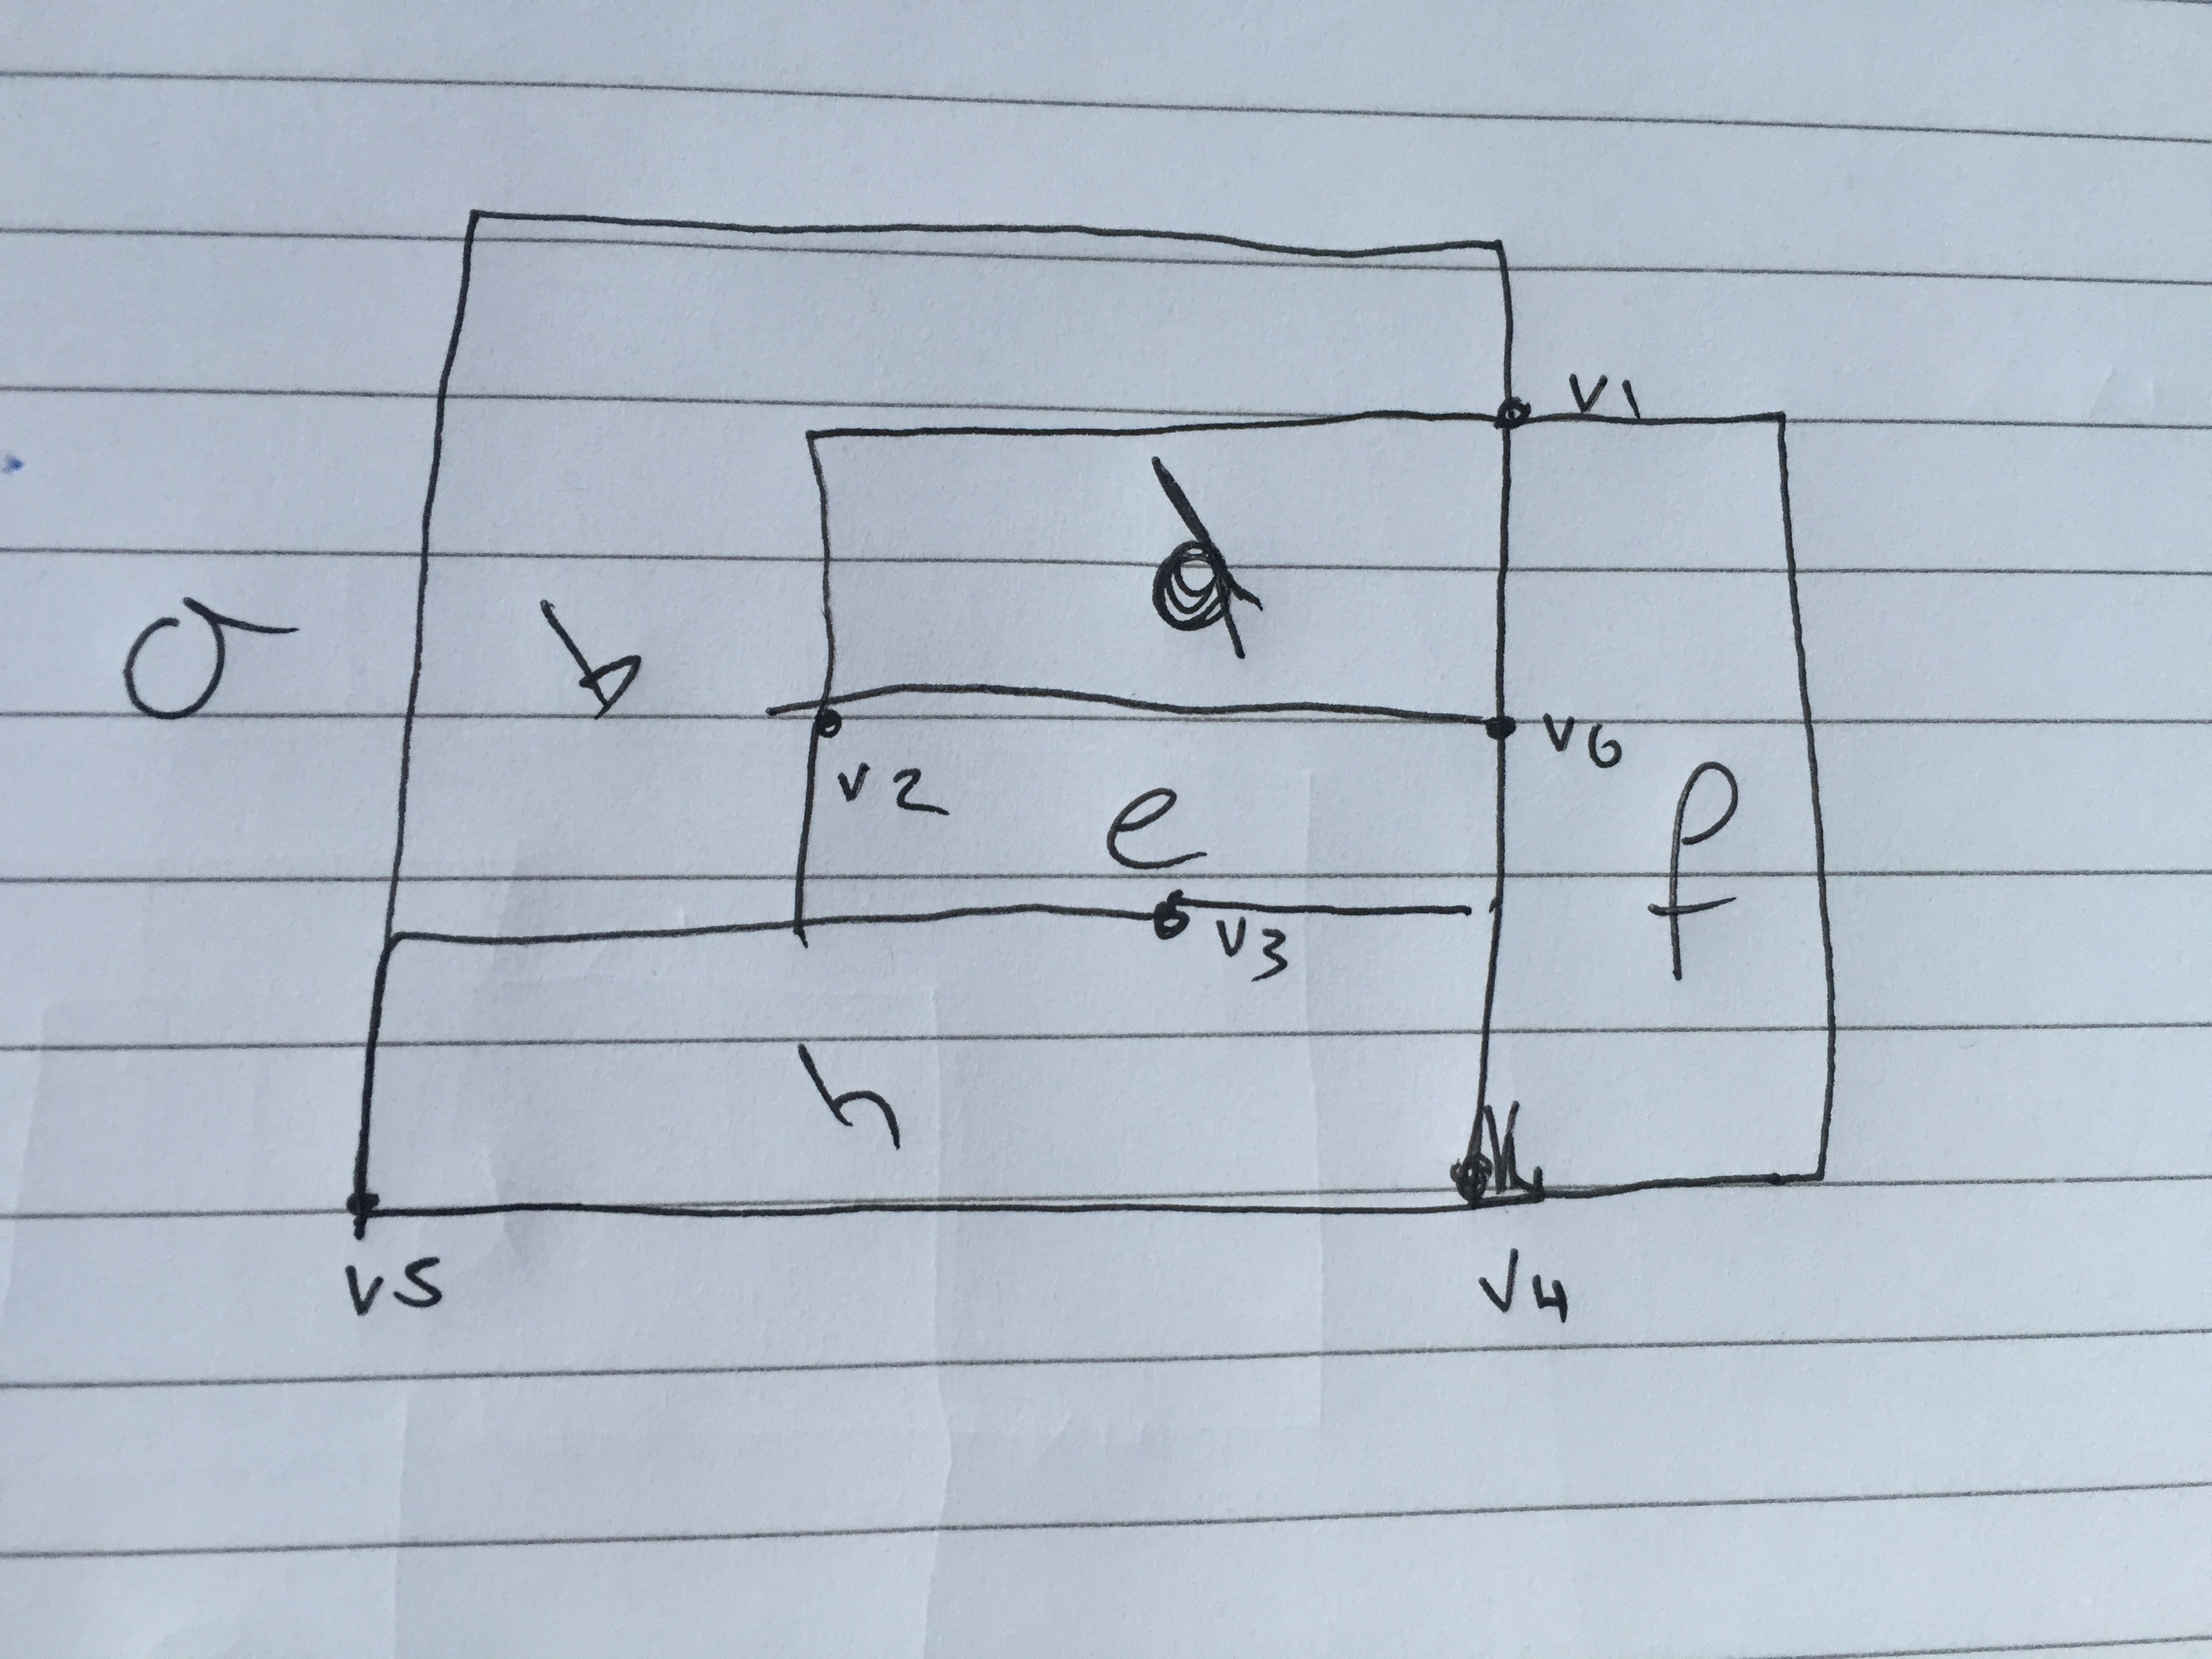
\includegraphics[scale=0.07]{images/planar-drawing.png}
  \caption{Rectilinear drawing of Graph 2(a) in assignment desc}
  \label{fig:rectidraw}
\end{figure}

\subsection{Exercise 2.2}
Let \(f_e\) be the external boundary cycle and \(B\) be the set of all boundaries. Inner turns (from \(x\) to \(y\)) are denoted by \(z_{xy}\) and outer turns (from \(y\) to \(x\)) are denoted by \(z{yx}\).
\begin{align}
  \forall f \in B \ f_e:&  \sum_{v} x_{vf_e} + \sum_{b\in B \ {f_e}} f_e - \ldots = -4\\
                        & \sum_{v} x_{vf} + \sum_{b\in B \ {f_e}} f - \ldots = 4 
\end{align}
